\documentclass{article}

\usepackage[utf8]{inputenc}
\usepackage[swedish]{babel}
\usepackage{color}
\usepackage{listings}
\usepackage{hyperref}
\usepackage[a4paper, margin=2.8cm]{geometry}
\usepackage{graphicx}
\hypersetup{
    colorlinks=true, %set true if you want colored links
    linktoc=all,     %set to all if you want both sections and subsections linked
    linkcolor=black,  %choose some color if you want links to stand out
}


\definecolor{codegreen}{rgb}{0,0.6,0}
\definecolor{codegray}{rgb}{0.5,0.5,0.5}
\definecolor{codepurple}{rgb}{0.58,0,0.82}
\definecolor{backcolour}{rgb}{0.95,0.95,0.92}
 
\lstdefinestyle{mystyle}{
    backgroundcolor=\color{backcolour},   
    commentstyle=\color{codegreen},
    keywordstyle=\color{magenta},
    numberstyle=\tiny\color{codegray},
    stringstyle=\color{codepurple},
    basicstyle=\footnotesize,
    breakatwhitespace=false,         
    breaklines=true,                 
    captionpos=b,                    
    keepspaces=true,                 
    %numbers=left,                    
    numbersep=5pt,                  
    showspaces=false,                
    showstringspaces=false,
    showtabs=false,                  
    tabsize=4
}
\lstdefinestyle{mystyle_numbers}{
    backgroundcolor=\color{backcolour},   
    commentstyle=\color{codegreen},
    keywordstyle=\color{magenta},
    numberstyle=\tiny\color{codegray},
    stringstyle=\color{codepurple},
    basicstyle=\footnotesize,
    breakatwhitespace=false,         
    breaklines=true,                 
    captionpos=b,                    
    keepspaces=true,                 
    numbers=left,                    
    numbersep=5pt,                  
    showspaces=false,                
    showstringspaces=false,
    showtabs=false,                  
    tabsize=4
}

\lstset{style=mystyle}

\author{Mattias Salo}
\title{Pong}

\begin{document}

\maketitle
\begin{figure}[h!]
	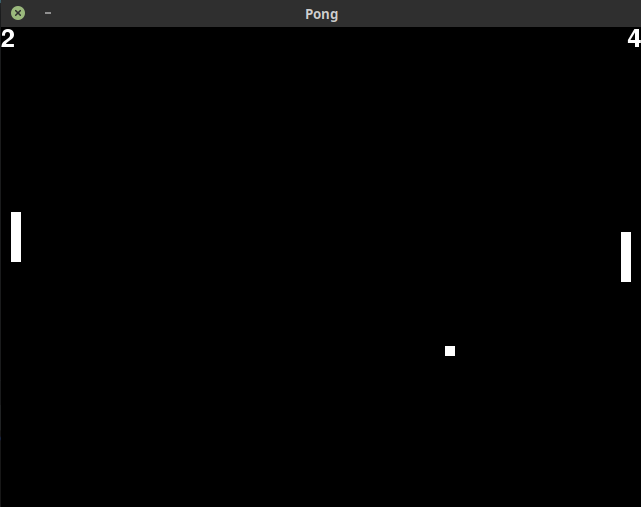
\includegraphics[width=\linewidth]{screenshot.png}
\end{figure}
\newpage

\tableofcontents

\newpage

\section{Introduktion}
Pong kom 1972 och var det första kommersiellt framgångsrika arkadspelet, där en fyrkant föreställande en boll ska bollas över nätet mellan två spelare som är utrustade med varsitt racket. Pong blev en succé och Atari, som tillverkade spelet, blev USA:s då snabbast växande företag.

\section{Sätt upp projektet}
Det första som ska göras är att bestämma alla de värden som vi ska använda som en bas att bygga vidare på. Detta är värden som inte ändras, såkallade konstanter (i Python skriver vi konstanter med stora bokstäver och understreck). Vi börjar med storleken på fönstret som spelet visas i, en bra storlek är 640 pixlar bred och 480 pixlar hög. Vi använder oftast engelska namn på de värdena, eftersom Python är gjort för att användas på engelska. Window betyder fönster, width betyder bredd, och height betyder höjd.
\begin{lstlisting}
WINDOW_WIDTH = 640
WINDOW_HEIGHT = 480
\end{lstlisting}
Vi vill även sätta ett värde på hur många gånger i sekunden som bildskärmen ska uppdateras (eftersom en rörlig bild egentligen är många bilder ändras väldigt snabbt). För att göra att det ser ut som att bollen rör på sig väldigt smidigt väljer vi ett värde på 60, den hastighet som många vanliga bildskärmar uppdaterar sina bilder med.
\begin{lstlisting}[language=Python]
FPS = 60
\end{lstlisting}
Där FPS står för ''Frames per Second'', eller bilder per sekund på svenska.\\
\\
Vi vill även lägga till biblioteket som gör det möjligt för oss att göra spelet och faktiskt visa upp det på skärmen, PyGame. Detta görs enklast genom att lägga till de här raderna högst upp i filen.
\begin{lstlisting}[language=Python]
import pygame
import sys
from pygame.locals import *
\end{lstlisting}
Vilka färger använder spelet? Eftersom spelet är så gammalt så är det bara två färger som används, svart och vit. Färger i PyGame skrivs med tre värden, som beskriver de tre färger som nästan alla skärmar är uppbyggda av, röd, grön och blå. De brukar förkortas RGB efter just de tre färgerna som används. Och hur får man då svart och vit genom att bara använda röd, grön och blå? Jo, det är så enkelt att svart är när ingen av de tre färgerna finns, och eftersom svart på engelska heter black blir konstanten för svart.
\begin{lstlisting}[language=Python]
BLACK = (0, 0, 0)
\end{lstlisting}
Men hur är det med vit? Vit är motsatsen till svart, det är när alla färger är ställda till max, vilket i det här fallet är 255. Därför ser konstanten för vit ut så här.
\begin{lstlisting}[language=Python]
WHITE = (255, 255, 255)
\end{lstlisting}
De här konstanterna lägger vi efter alla andra konstanter.\\
\\
Nu är det dags att skriva lite kod som faktiskt gör någonting. Vi ska skriva den kodsnutten som vi vill ska köras först i hela programmet. För detta vill vi skapa en funktion som heter main, där main i princip betyder huvud, eftersom det är därifrån programmet styrs. I main lägger vi till lite kod för att starta pygame och klockan som håller reda på hur många bilder per sekund som spelet ska visa.
\begin{lstlisting}[language=Python]
def main():
    pygame.init()
    fps_clock = pygame.time.Clock()
    display_surf = pygame.display.set_mode((WINDOW_WIDTH, WINDOW_HEIGHT))
    pygame.display.set_caption("Pong")

    while True:
        # Koden dar spelet ska koras
\end{lstlisting}
display\_surf är här det som vi ska använda för att måla vår spelplan på. pygame.display.set\_caption(''Pong'') är det som gör att det kommer stå Pong på vårt fönster. Där det står while True: är där vår loop för att styra spelet är, (som vi kommer börja skriva på snart) den loopen kommer köra ett helt spel av Pong. När den är klar kommer ett nytt spel att börja (eftersom den här loopen är en evighetsloop).\\
\\
Nu kan vi börja skriva på funktionen run\_game(display\_surf, fps\_clock) som faktiskt ska köra en hel omgång av Pong, det är här vi ska skriva allt som gör att spelet fungerar. Till en början ska vi se till att visa en bakgrund, och i Pong är den ju svart. Vi skriver alltså en funktion som ser ut så här.
\begin{lstlisting}[language=Python]
def run_game(display_surf, fps_clock):
    while True:  # main game loop
        display_surf.fill(BLACK)
        fps_clock.tick(FPS)
\end{lstlisting}
Vi kan då se att vi även här använder en evighetsloop, men där varje omgång i loopen inte beskriver ett helt spel men istället en bild av spelet. fps\_clock.tick(FPS) är den raden kod som gör att precis 60 bilder per sekund ska visas, utan den skulle spelet gå jättesnabbt. display\_surf.fill(BLACK) är den raden kod som gör att vi faktiskt ritar upp en svart bakgrund, eller rättare sagt fyller hela skärmen med färgen svart. För att köra den här koden måste den läggas till i main(), inuti evighetsloopen alltså.
\begin{lstlisting}[language=Python]
	while True:
		run_game(display_surf, fps_clock)
\end{lstlisting}
Innan vi kan starta spelet är det endast en till kodsnutt som behöver läggas till.
\begin{lstlisting}[language=Python]
if __name__ == "__main__":
	main()
\end{lstlisting}
Den här kodsnutten ska alltid ligga längst ner i Python-filen, den bestämmer vilken funktion som ska köras när programmet startar. Eftersom vi har sagt att vår main() funktion ska startas först skriver vi in den.\\
\\
Om du startar filen nu kommer du kunna se svart fönster med titeln Pong, coolt eller hur!\\
\\
Om den inte visar det kan du kolla på följande kodsnutt, vilket är hur din fil kan se ut för att det ska fungera.
\begin{lstlisting}[language=Python, style=mystyle_numbers]
import pygame
import sys
from pygame.locals import *

WINDOW_WIDTH = 640
WINDOW_HEIGHT = 480
FPS = 60

BLACK = (0, 0, 0)
WHITE = (255, 255, 255)


def main():
	pygame.init()
	fps_clock = pygame.time.Clock()
	display_surf = pygame.display.set_mode((WINDOW_WIDTH, WINDOW_HEIGHT))
	pygame.display.set_caption("Pong")
	
	while True:
		run_game(display_surf, fps_clock)

		
def run_game(display_surf, fps_clock):
	while True: # main game loop
		display_surf.fill(BLACK)
		fps_clock.tick(FPS)
		

if __name__ == "__main__":
	main()
\end{lstlisting}


\newpage
\lstinputlisting[language=Python, style=mystyle_numbers]{main.py}


\end{document}
